\documentclass[a4paper,norsk]{article}
\usepackage{preamble}
\usepackage{tabu}
\usepackage{color, colortbl}
\definecolor{LightCyan}{rgb}{0.88,1,1}


\begin{document}
\maketitle

\section{Exercise 1}
In these set of exercises we will study the Stokes problem defined as 
\begin{align*}
-\Delta u + \nabla p = f \hspace{2mm} \text{in} \hspace{2mm} \Omega \\
\nabla \cdot v = 0 \hspace{2mm} \text{in} \hspace{2mm} \partial\Omega \\
u = g \hspace{2mm} \text{in} \hspace{2mm} \partial\Omega_N \\
\frac{\partial u}{\partial x} - pn = h \hspace{2mm} \text{in} \hspace{2mm} \partial\Omega_N\\
\end{align*}

First off we will define the weak formulation for the stokes problem. Let u $\in H_{D,g}^1$ and $p \in L^2$. Then
the stokes problem can be defined as 
\begin{align*}
a(u, v) + b(p, v) = f(v) \hspace{2mm} v \in H_{D,0}^1 \\
b(q, u) = 0 \hspace{2mm} q \in L^2 
\end{align*}
Where a and b defines the bilinear form, and f defines the linear form as

\begin{align*}
a(u, v) = \int \nabla u : \nabla v \hspace{1mm} dx \\
b(p, v) = \int p \nabla \cdot v \hspace{1mm} dx \\
f(v) = \int f v \hspace{1mm} dx + \int_{\Omega_N} h v \hspace{1mm} ds
\end{align*}

Further we will define to properties which will be usefull for solving the exercises \newline
\textbf{Cauchy-Schwarts inequality} \\
Let V be a inner product space, then
\begin{align*}
 |\langle u \,, v \rangle| \hspace{1mm} \leq \hspace{1mm} ||u|| \cdot ||w|| \hspace{2mm} \forall \hspace{1mm} v,q \in V
\end{align*}
\newline
\textbf{Poincare's Inequality}
Let $v \in H_0^1(\Omega)$
\begin{align*}
||v||_{L^2(\Omega)} \leq C |v|_{H^1} (\Omega) 
\end{align*}

\newpage
\subsection*{Exercise 7.1}
In this section we are to prove the conditions (7.14-7.16) from the course lecturenotes. 
Starting off with the first 
\textbf{Condition 7.14}
\begin{align*}
a(u_h, v_h) \leq C_1 ||u_n||_{V_n} ||v_n||_{V_n} \hspace{2mm} \forall u_n, v_n \in V_n
\end{align*}
As for in all of these conditions we will assume that $V_h \in H_0^1$, and for later conditions that$Q_h \in L^2$.
\newline
First off we write out the term $a(u_h, v_h)$, and we observe we can use the Cauchy-Schwarts inequality since
V is an inner product space. 
\begin{align*}
a(u_h, v_h) = \int_\Omega \nabla u_h : \nabla v_h \hspace{1mm} dx  = \langle \nabla u_h \,, \nabla v_h \rangle \\
\langle \nabla u_h \,, \nabla v_h \rangle \leq |\langle \nabla u_h \,, \nabla v_h \rangle|_0 \leq ||\nabla u_h||\cdot ||\nabla v_h||
\end{align*}
Now since we have defined that $u_h, v_h \in V_h \in H_0^1$ we can use the Poincare inequality. First we observe that

\begin{align*}
||\nabla u_h ||^2_{L^2} \leq ||u_h||^2_{H^1} = ||u_h||^2_{L^2} + ||\nabla u_h||^2_{L^2} \leq C_1 |u_h|^2_{H_1} +  ||\nabla u_h||^2_{L^2} =
C_1 ||\nabla u_h||^2_{L2} +  ||\nabla u_h||^2_{L^2} \\
(C_1 + 1) ||\nabla u_h||^2_{L2} \leq D ||u_h||^2_{H^1} 
\end{align*}



\textbf{Condition 7.14}
\begin{align*}
b(u_h, q_h) \leq C_2 ||u_h||_{V_h} ||q_h||_{Q_h} \hspace{2mm}  V_h \in H_0^1, \hspace{2mm} Q_h \in L^2,
\end{align*}
By direct insertion we get 

\begin{align*}
b(u_h, q_h) = \int p \nabla \cdot v \hspace{1mm} dx = \langle p \,, \nabla \cdot u \rangle \leq | \langle p \,, \nabla \cdot u \rangle |_0
\end{align*}
Using the Cauchy-Schwarts inequality we can show that
\begin{align*}
| \langle q \,, \nabla \cdot u \rangle | \leq ||q||_0 \cdot ||\nabla \cdot u||_0
\end{align*}
Hence, it holds to show that
\begin{align*}
  ||q||_0 \cdot ||\nabla \cdot u||_0 \leq C_2 ||u_h||_{1} ||q_h||_{0} \\
  ||\nabla \cdot u||_0 \leq C_2 ||u_h||_{1} 
\end{align*}
We choose square the left side of the inequality and expand the norm, in hope of finding a term to
determine the upper bound of b. Applying the poincare inequality on line 2, we can determine that the bound must be
determined by some constant $C_2$
\begin{align*}
||\nabla \cdot u||_0^2 \leq ||u||_1^2 = ||u||_0^2 + ||\nabla u ||_0^2 \\
||u||_0^2 + ||\nabla u ||_0^2 \leq C_2^2 |u|_1 + ||\nabla u||_0^2 = (C_2^2 + 1)||\nabla u ||_0^2 = C_2^2||\nabla u ||_0^2
\end{align*}
Hence, to show the implied boundedness of b, it holds to show $||\nabla \cdot u||_0^2 \leq (C_2^2 + 1)||\nabla u ||_0^2$
For simplicity we write out the terms for the $R^2$ case, but the same proof can be showed for the general case $R^n$. 

\begin{align*}
 ||\nabla \cdot u||_0^2 = \int \big(\frac{\partial^2 u}{\partial x^2} + \frac{\partial^2 v}{\partial y^2}\big)^2 \hspace{1mm} dx \\
 ||\nabla u||_0^2 = \int \big(\frac{\partial^2 u}{\partial x^2}\big)^2 + \big(\frac{\partial^2 u}{\partial y^2} \big)^2 + 
 \big(\frac{\partial^2 v}{\partial x^2} \big)^2 + \big( \frac{\partial^2 v}{\partial y^2} \big)^2 \hspace{1mm} dx
\end{align*}
Remembering that since we are in a normed vector space V, the triangle inequality holds.
\begin{align*}
||x + y || \leq ||x|| + ||y|| \hspace{2mm} \forall x,y \in V
\end{align*}
Rearrangeing the terms we observe that 
\begin{align*}
 ||\nabla \cdot u||_0^2 = \int \big(\frac{\partial^2 u}{\partial x^2} + \frac{\partial^2 v}{\partial y^2}\big)^2 \hspace{1mm} dx \\
 ||\nabla u||_0^2 = \int \big(\frac{\partial^2 u}{\partial x^2}\big)^2 
 +  \big( \frac{\partial^2 v}{\partial y^2} \big)^2 \hspace{1mm} dx
 + \int \big(\frac{\partial^2 v}{\partial x^2} \big)^2 + 
  \big(\frac{\partial^2 u}{\partial y^2} \big)^2  \hspace{1mm} dx \\
  \sqrt{ \int \big(\frac{\partial^2 u}{\partial x^2} + \frac{\partial^2 v}{\partial y^2}\big)^2 \hspace{1mm} dx }\leq 
 \sqrt{ \int \big(\frac{\partial^2 u}{\partial x^2}\big)^2} 
 + \sqrt{ \big( \frac{\partial^2 v}{\partial y^2} \big)^2 \hspace{1mm} dx }
\end{align*}
Hence $||\nabla \cdot u||_0^2 \leq C_2^2 ||\nabla u ||_0^2$, and the inequality holds. 

\textbf{Condition 7.16, Coersivity of a}
\begin{align*}
 a(u_h, u_h) \geq C_3 ||u_h||_{V_h}^2 \hspace{2mm} \forall u_h \in V_h
\end{align*}
Expanding the $H^1$ norm of $u_h$, and applying the Cauchy-Schwarts inequality we find the relations

\begin{align*}
||u_h||_1^2 = ||u_h||_0^2 + ||\nabla u_h||_0^2 \leq C|u_h|_1^2 + ||\nabla u_h||_0^2 \\
= C||\nabla u_h||_0^2 + ||\nabla u_h||_0^2 = \big(C + 1\big)||\nabla u_h||_0^2 = C_3 ||\nabla u_h||_0^2 \\
\end{align*}
Dividing the constant on both sides of the inequality and let $C_3 = 1/C_3$ we get our final result which proofs the coersivity of a
\begin{align*}
C_3||u_h||_1^2 \leq ||\nabla u_h||_0^2 = \int \nabla u_h : \nabla u_h \hspace{1mm} dx = a(u_h, u_h)
\end{align*}

\newpage
\subsection{Exercise 7.6}
Looking on the poiseuille flow, we are to investigate if the anticipated convergence rates applies for the problem

\begin{align*}
-\Delta u - \nabla p = f \hspace{2mm} \text{in} \hspace{2mm} \Omega \\
\nabla \cdot v = 0 \hspace{2mm} \text{in} \hspace{2mm} \partial\Omega \\
\end{align*}
We will make use of the "manufactured solution" approach defining the analytical solution in $\Omega$ and finding the appropriate
soruce function as

\begin{align*}
 u = (sin(\pi y), cos(\pi x)); \hspace{4mm} p = sin(2 \pi x) \\
 f = (\pi^2 sin(\pi y) - 2 \pi cos(2 \pi x), \pi^2 cos(\pi x)) 
\end{align*}

We will this exercise examinate the error estimate 
\begin{align*}
 ||u - u_h||_1 + ||p - p_h||_0 \leq Ch^k||u||_{k+1} + Dh^{l+1} ||p||{l+1}
\end{align*}
Where \textit{k}, \textit{l} denotes the polynomial degree of the velocity and pressure. The error estimate will be
examined using $(P_4 - P_3)$, $(P_4 - P_2)$, $(P_3 - P_2)$ and $(P_3 - P_1)$ elements for velocity and pressure accordingly. 
The problem will be solved on a UnitSquareMesh(N, N), for $N = [8, 16, 32, 64]$. Order of convergence is calculated for each choice
of elements, between to neighbouring N values defined as

\begin{align*}
 r  = \frac{log \big( \frac{E[i+1]}{E[i]} \big)} {log \big( \frac{(h[i+1]}{h[i]} \big)}
\end{align*}
Where E is a list of errornorms and h is a list of the facetlength in the mesh defined as $\frac{1}{N}$



\begin{table}[ht]
\caption {Convergence rate velocity, $E = ||u-u_h||_1$} 
\centering
\begin{tabular}{c|ccccccc}
\hline
\rowcolor{LightCyan}
N  & Conv 4 to 8  &  Conv 8 to 16  &  Conv 16 to 32 &  Conv 32 to 64 \\  
\hline
4-3   &     4.53315  &       4.2951   &        4.11514  & 4.03954 \\ \hline
4-2    &    2.6871   &       2.88045  &        2.96138 & 2.98766 \\ \hline
3-2    &    2.57912  &       2.84778  &        2.9518 & 2.98466 \\ \hline
3-1    &    2.17924  &       2.08939  &        2.04646 & 2.02452 \\
\hline
\end{tabular}
\end{table}
       

\begin{table}[ht]
\caption {Convergence rate velocity, $E = ||p-p_h||_0$} 
\centering
\begin{tabular}{c|ccccccc}
\hline
\rowcolor{LightCyan}
N  & Conv 4 to 8  &  Conv 8 to 16  &  Conv 16 to 32 &  Conv 32 to 64\\
\hline
4-3   &     4.22147   &      4.08419   &       4.02915 & 4.01063  \\ \hline
4-2   &     2.71627   &      2.89978   &       2.97342 & 2.99382  \\ \hline 
3-2   &     2.71694   &      2.90114   &       2.97394 & 2.99397   \\ \hline 
3-1   &     2.35349   &      2.19402   &       2.09554 & 2.04362   \\ 
\hline
\end{tabular}
\end{table}

To describe these results we have to take a closer look on the error estimate. Let us choose the dataset from the $(P_4 - P_3)$
computation. For $k=4$ and $p=3$ we get.  

\begin{align*}
 ||u - u_h||_1 + ||p - p_h||_0 \leq Ch^4||u||_{5} + Dh^{4} ||p||{4}
\end{align*}
Observing that C,D, $||u||_{5}$ and $||p||_{4}$ are some constants and will not effect the trend of the error estimate, we see that
the error is limited to $h^4$, both for the velocity and pressure norm. From our result this seems reasonable as we can see the order of convergence
approach 4.

What  about if we choose some elements which differ in degree by 2? Let's choose the $(P_4 - P_2$ computation and see what is going on. Our error estimate then yields
\begin{align*}
 ||u - u_h||_1 + ||p - p_h||_0 \leq Ch^4||u||_{5} + Dh^{3} ||p||_{3}
\end{align*}
Now as the velocity norm on the right side of the inequality is dominated by the h term, we obsere that this term will go faster to zero than the pressure norm. Hence our 
calculations should be dominated by the pressure norm. From this logic we would expect the order of convergence to be limited by 3. As we can see from the numerical results, this seems 
legit as we can see that the rate of convergence approaches 3 as the mesh gets finer. 


\begin{figure}[h!]
	\centering
	\caption*{loglogplot}
	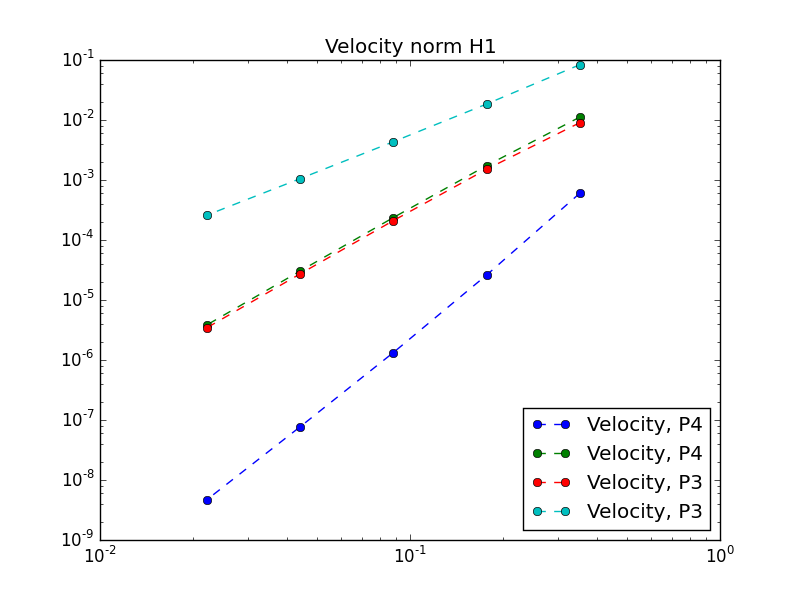
\includegraphics[scale=0.32]{velocity.png}
		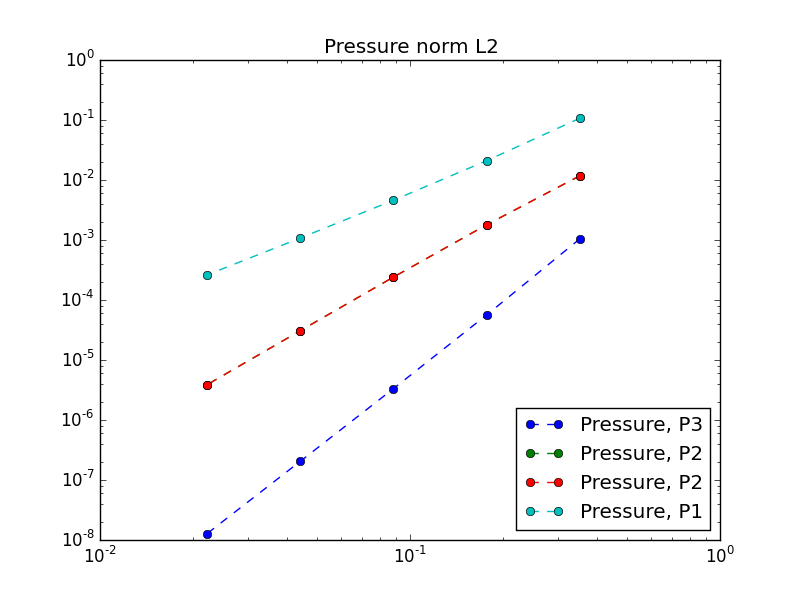
\includegraphics[scale=0.32]{pressure.png}
\end{figure}

\begin{figure}[h!]
	\centering
	\caption*{loglogplot}
	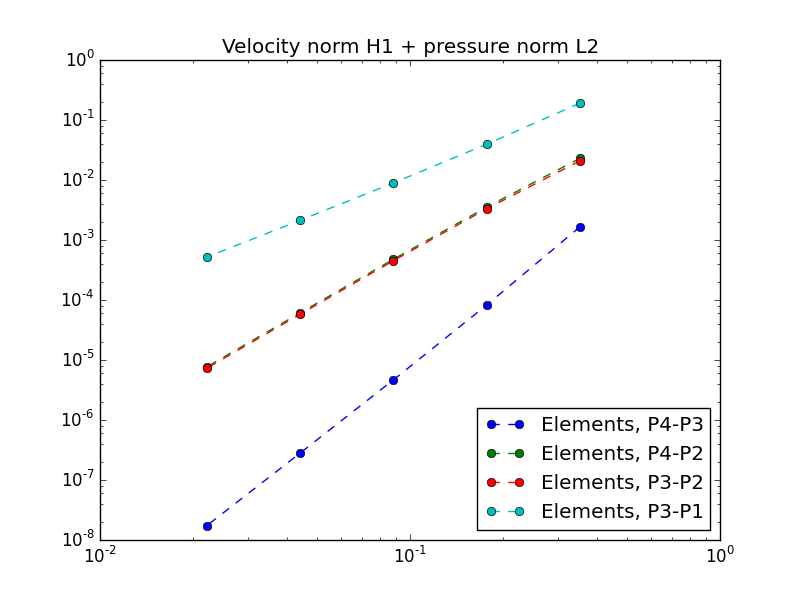
\includegraphics[scale=0.4]{comb.png}
\end{figure}

\newpage
\subsection{Exercise 7.7}
In this exercise we where to calculate the order of convergence for the shear stress in the same domain presented en exercise 7.6.
Let \textit{P} denote the stress tensor. The wall stress on a surface in the domain is given by $\textit{P} \cdot \textbf{n}$, where \textbf{n} is the normal vector 
pointing perpendicular to the surface out of the domain. Hence we have the following relations

\begin{align*}
 &\textbf{\textit{P}}_n = \textit{P} \cdot \textbf{n} \hspace{12mm} \text{Shear stress} \\
	&P_{nn} = \textbf{n} \cdot \textbf{\textit{P}}_n \hspace{8mm} \text{Normal stress component} \\
	&P_{nt} = |\textbf{\textit{P}}_n \times \textbf{n}| \hspace{5mm} \text{Tangential stress component}
	\end{align*}

	In this exercise we are interested in the wall shear stress, hence we will for this time focus on the tagential stress.

	
\end{document}
